% MICA final report — evidence figures (all numbers from banked artifacts, 2026-07-19)
% Compile: pdflatex evidence_figures.tex   (needs pgfplots >= 1.17)
% Each figure is self-contained; copy any single figure environment into the report.
\documentclass[11pt]{article}
\usepackage[margin=1in]{geometry}
\usepackage{amsmath}
\usepackage{booktabs}
\usepackage{pgfplots}
\pgfplotsset{compat=1.17,
  every node near coord/.append style={/pgf/number format/fixed,
    /pgf/number format/precision=3}}
\usepackage{caption}
\definecolor{micablue}{RGB}{46,110,180}
\definecolor{micagray}{RGB}{140,140,140}
\definecolor{micagreen}{RGB}{60,145,90}
\definecolor{micared}{RGB}{180,70,60}

\begin{document}

\section*{MICA --- evidence figures}

\subsection*{Where each number comes from: written rules, learning, or both}

The system has two kinds of parts, and every figure below says which kind
produced its numbers. \textbf{Hand-rule} parts are instructions a person wrote
down --- ``compare the structure to these known shapes,'' ``only act when
confidence passes this bar.'' They do exactly what they were told, nothing
more. \textbf{Observation} parts were not told what to do --- they learned by
watching recordings of a person building, the way one learns a coworker's
habits. \textbf{Both} means a hand-written frame carrying learned content
inside it.

\begin{center}\small
\begin{tabular}{llll}
\toprule
Figure / finding & written-rule part & learned-by-watching part & type \\
\midrule
Fig.~1 five designs & the losing baseline itself; & the winner's evidence & \textbf{both}\\
 & the belief-update rule & judgments & \\
Fig.~2 real pretraining & data tidying only & teacher: the human's own & \textbf{obs.}\\
 & & recorded next actions & \\
Fig.~3 disputed labels & sorting sessions into groups & the trained parts; builder's & \textbf{both}\\
 & & label as the answer key & \\
Fig.~4 seeing = knowing & counting seen blocks & the shape representation & \textbf{obs.}\\
Fig.~5 live case study & the belief-update rule & evidence judgments & \textbf{both}\\
Fig.~6 move prediction & the definition of ``right'' & the predictor, end to end & \textbf{obs.}\\
structure checker & entirely written rules & --- & \textbf{hand}\\
safety gate + consent & entirely written rules (by design) & --- & \textbf{hand}\\
\bottomrule
\end{tabular}
\end{center}

The split is itself a result. \textbf{Hand-rule parts are where trust lives}:
on builds they were written for, they are perfect (the matcher scores 1.0 on
the known-truth corpus) and anyone can read exactly why they answered as they
did --- but on new, unplanned builds they collapse (0.042 in Fig.~1), and that
collapse was measured, not assumed. \textbf{Learned parts are where
flexibility lives}: they keep working on builds nothing was written for
(0.375), and they get better simply by watching more (Figs.~2--4). The system
divides the work accordingly: \emph{written rules decide when it is safe to
speak or act}; \emph{learned parts do the watching and predicting}. Fig.~1 is
the head-to-head test behind that division --- rules alone fail exactly where
real, unscripted work happens.

% ---------------------------------------------------------------- Figure 1
\begin{figure}[h]
\centering
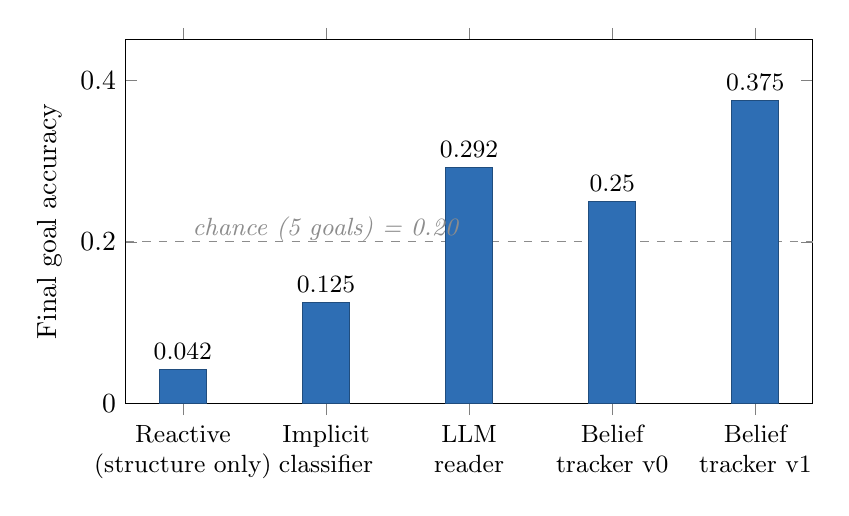
\begin{tikzpicture}
\begin{axis}[
  width=0.85\textwidth, height=6.2cm,
  ybar, bar width=17pt,
  ymin=0, ymax=0.45,
  ylabel={Final goal accuracy},
  symbolic x coords={Reactive, Implicit, LLM reader, Belief v0, Belief v1},
  xtick=data,
  xticklabels={Reactive\\(structure only), Implicit\\classifier, LLM\\reader, Belief\\tracker v0, Belief\\tracker v1},
  x tick label style={font=\small, align=center},
  nodes near coords, nodes near coords style={font=\small},
  extra y ticks={0.2}, extra y tick labels={},
  extra tick style={grid=major, grid style={dashed, micagray}},
]
\addplot[fill=micablue, draw=micablue!70!black] coordinates {
  (Reactive, 0.042)
  (Implicit, 0.125)
  (LLM reader, 0.292)
  (Belief v0, 0.250)
  (Belief v1, 0.375)
};
\node[anchor=west, font=\small\itshape, color=micagray]
  at (axis cs:Reactive, 0.215) {chance (5 goals) = 0.20};
\end{axis}
\end{tikzpicture}
\caption{\textbf{Guessing what the builder is making: five designs, one test.}
Five different designs watched the same 24 recorded building sessions --- real,
free-form builds that none of them had ever seen --- and each had to name what
the builder was making, out of five goal categories. Each bar is the share of
sessions a design got right; random guessing scores 0.20 (dashed line). The
leftmost design, which skips inference and just compares the structure to a
library of known shapes, scores 0.042 --- \emph{worse} than guessing, because
free-form builds match nothing in its library. The design that maintains a
running belief about the builder's intention scores 0.375, nine times better.
Since every design saw identical input, the gap can only come from the
inference itself. (Comparison run of 2026-07-19.)
\textit{Source: BOTH --- the failing baseline is the hand-written rules; the
winner is learned content inside a hand-written frame.}}
\end{figure}

% ---------------------------------------------------------------- Figure 2
\begin{figure}[h]
\centering
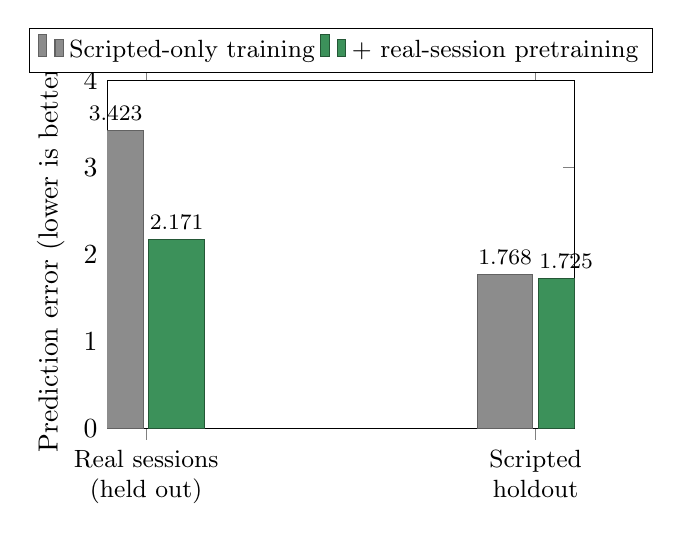
\begin{tikzpicture}
\begin{axis}[
  width=0.62\textwidth, height=6cm,
  ybar, bar width=20pt,
  ymin=0, ymax=4.0,
  ylabel={Prediction error (lower is better)},
  symbolic x coords={Real sessions, Scripted holdout},
  xtick=data,
  xticklabels={Real sessions\\(held out), Scripted\\holdout},
  x tick label style={font=\small, align=center},
  legend style={font=\small, at={(0.5,1.02)}, anchor=south, legend columns=2},
  nodes near coords, nodes near coords style={font=\footnotesize},
]
\addplot[fill=micagray, draw=micagray!70!black] coordinates {
  (Real sessions, 3.4228) (Scripted holdout, 1.7683) };
\addplot[fill=micagreen, draw=micagreen!60!black] coordinates {
  (Real sessions, 2.1708) (Scripted holdout, 1.7246) };
\legend{Scripted-only training, + real-session pretraining}
\end{axis}
\end{tikzpicture}
\caption{\textbf{A model trained on artificial data struggles with real people
--- until it watches real recordings.} The bars show prediction error when the
model guesses a builder's next action: lower is better. Trained only on
computer-generated example builds (gray), the model predicts artificial
builders well but real ones poorly --- the left gray bar towers over the right
one. Letting it first watch real recorded sessions (green) cuts its error on
real builders by 37\%. The key: this extra training needed \emph{no labels at
all}. The model simply watches a recording and tries to guess each next
action, so even sessions whose goal was disputed or unidentifiable could
teach it --- a doubtful label cannot mislead training that uses no labels.
The test sessions were locked in before the experiment ran.
\textit{Source: OBSERVATION --- the teacher is the human's own recorded next
actions; written rules only tidy the data.}}
\end{figure}

% ---------------------------------------------------------------- Figure 3
\begin{figure}[h]
\centering
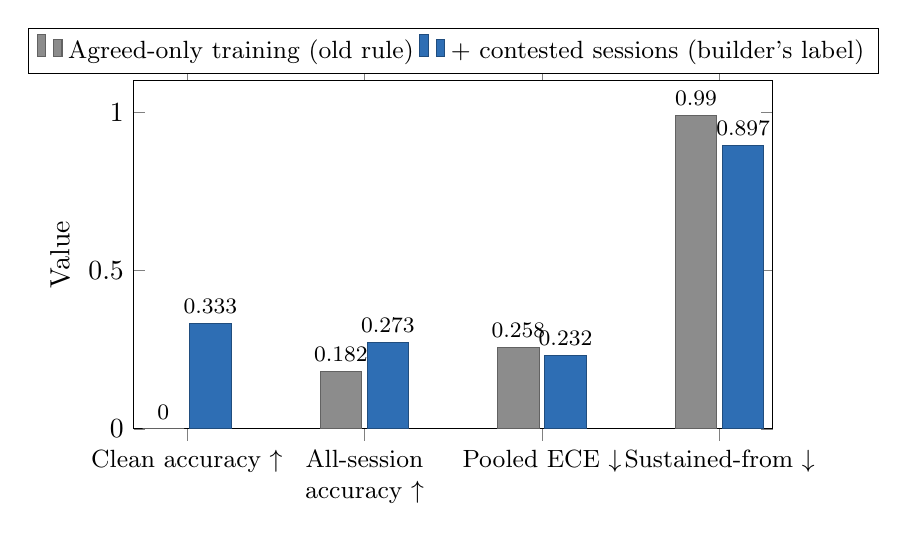
\begin{tikzpicture}
\begin{axis}[
  width=0.8\textwidth, height=6cm,
  ybar, bar width=15pt,
  ymin=0, ymax=1.1,
  ylabel={Value},
  symbolic x coords={CleanAcc, AllAcc, ECE, Sustained},
  xtick=data,
  xticklabels={Clean accuracy $\uparrow$, All-session accuracy $\uparrow$, Pooled ECE $\downarrow$, Sustained-from $\downarrow$},
  x tick label style={font=\small, text width=2.6cm, align=center},
  legend style={font=\small, at={(0.5,1.02)}, anchor=south, legend columns=2},
  nodes near coords, nodes near coords style={font=\footnotesize},
]
\addplot[fill=micagray, draw=micagray!70!black] coordinates {
  (CleanAcc, 0.000) (AllAcc, 0.182) (ECE, 0.2584) (Sustained, 0.990) };
\addplot[fill=micablue, draw=micablue!70!black] coordinates {
  (CleanAcc, 0.333) (AllAcc, 0.273) (ECE, 0.2324) (Sustained, 0.897) };
\legend{Agreed-only training (old rule), + contested sessions (builder's label)}
\end{axis}
\end{tikzpicture}
\caption{\textbf{When human and machine disagree about a session, trust the
human.} Some recorded sessions are ``disputed'': the builder said one goal,
the automatic checker said another. The old rule kept such sessions out of
training (gray bars); the new rule trains on them, taking the builder's word
as the truth (blue bars). On a shared test set that neither version trained
on, keeping them improved all four measures: accuracy on cleanly-labeled
sessions (0 $\to$ 0.33), accuracy across all sessions, how well stated
confidence matches actual correctness (ECE; lower is better), and how early
in a build the right answer locks in and stays (lower is earlier). Honesty
note: an earlier run of this same experiment found the \emph{opposite}; a
data flaw was found and repaired, the experiment was rerun, and the reversal
is on the record --- and re-checked at every retrain. The test set is small
(11 sessions).
\textit{Source: BOTH --- learned parts trained on watched sessions, with the
builder's own label as the answer key; written rules only sort sessions into
groups.}}
\end{figure}

% ---------------------------------------------------------------- Figure 4
\begin{figure}[h]
\centering
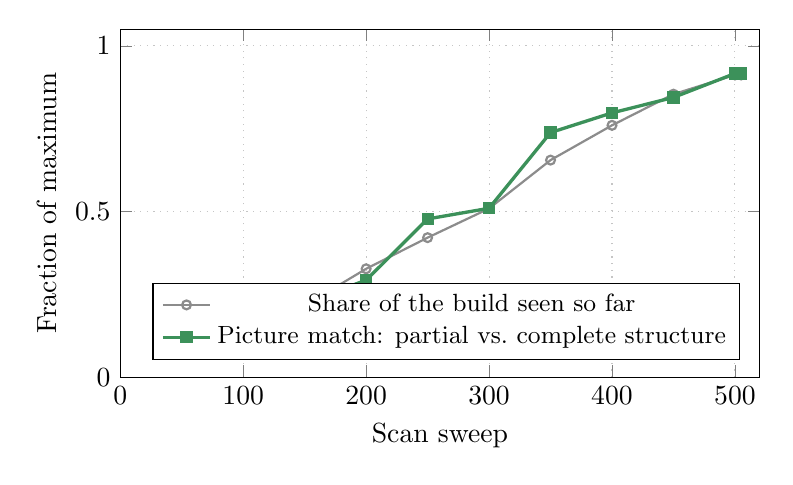
\begin{tikzpicture}
\begin{axis}[
  width=0.8\textwidth, height=6cm,
  xmin=0, xmax=520, ymin=0, ymax=1.05,
  xlabel={Scan sweep}, ylabel={Fraction of maximum},
  legend style={font=\small, at={(0.97,0.05)}, anchor=south east},
  grid=major, grid style={dotted, micagray!50},
]
% coverage: built_seen / 171
\addplot[micagray, thick, mark=o, mark size=1.6pt] coordinates {
  (100,0.094) (150,0.216) (200,0.327) (250,0.421) (300,0.509)
  (350,0.655) (400,0.760) (450,0.854) (500,0.912) (505,0.912) };
% cosine vs exact h3d
\addplot[micagreen, very thick, mark=square*, mark size=1.6pt] coordinates {
  (100,0.1165) (150,0.2241) (200,0.2927) (250,0.4775) (300,0.5097)
  (350,0.7382) (400,0.7976) (450,0.8442) (500,0.9164) (505,0.9164) };
\legend{Share of the build seen so far, Picture match: partial vs.\ complete structure}
\end{axis}
\end{tikzpicture}
\caption{\textbf{Seeing more means understanding more.} The agent walks around
the builder's work and can only know what its own eyes have passed over ---
it gets no map, no list of blocks from the game. The gray line shows how much
of the build it has seen so far; the green line asks a harder question: does
its mental picture of the \emph{partial} structure it has seen match the
picture it would form of the \emph{complete} structure? (1.0 = identical.)
The two lines rise together: by the time 91\% of the build has been seen, the
match reaches 0.92 --- watching most of the build is nearly as good as seeing
all of it. (One fully instrumented session,
\texttt{fabric-20260719-052914}.)
\textit{Source: OBSERVATION --- the ``mental picture'' is a learned shape
representation; only the seen-block counting is hand bookkeeping.}}
\end{figure}

% ---------------------------------------------------------------- Figure 5
\begin{figure}[h]
\centering
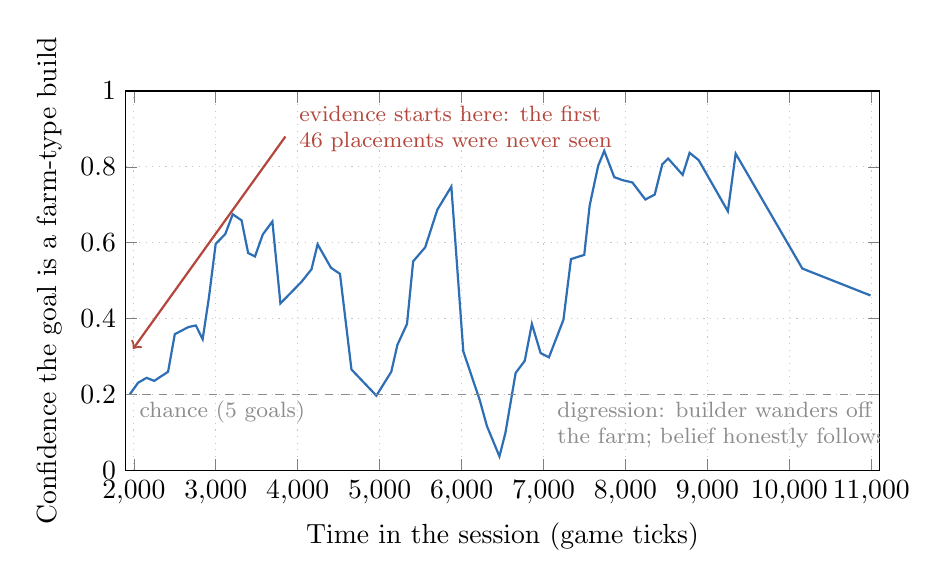
\begin{tikzpicture}
\begin{axis}[
  width=0.92\textwidth, height=6.4cm,
  xmin=1900, xmax=11100, ymin=0, ymax=1.0,
  xlabel={Time in the session (game ticks)},
  ylabel={Confidence the goal is a farm-type build},
  scaled x ticks=false, xticklabel style={/pgf/number format/fixed},
  grid=major, grid style={dotted, micagray!50},
]
\addplot[micablue, thick] coordinates {
  (1952,0.201) (2052,0.231) (2156,0.244) (2249,0.236) (2418,0.260)
  (2500,0.359) (2668,0.378) (2757,0.382) (2840,0.346) (2916,0.455)
  (2999,0.597) (3116,0.623) (3207,0.675) (3315,0.659) (3395,0.573)
  (3479,0.564) (3574,0.622) (3691,0.656) (3789,0.440) (4046,0.497)
  (4168,0.530) (4243,0.596) (4406,0.534) (4516,0.518) (4656,0.266)
  (4960,0.197) (5142,0.260) (5217,0.331) (5334,0.386) (5409,0.551)
  (5556,0.588) (5704,0.687) (5875,0.748) (6021,0.314) (6222,0.185)
  (6309,0.117) (6462,0.037) (6535,0.099) (6660,0.257) (6771,0.289)
  (6858,0.386) (6965,0.309) (7066,0.298) (7243,0.397) (7335,0.557)
  (7497,0.568) (7563,0.698) (7667,0.803) (7741,0.842) (7863,0.773)
  (7964,0.765) (8084,0.759) (8243,0.714) (8357,0.727) (8450,0.807)
  (8521,0.822) (8698,0.779) (8783,0.837) (8893,0.818) (9250,0.683)
  (9345,0.835) (10159,0.532) (10991,0.461)
};
\addplot[micagray, dashed, domain=1900:11100] {0.2};
\node[anchor=west, font=\footnotesize, color=micagray] at (axis cs:1950,0.155)
  {chance (5 goals)};
\node[anchor=west, font=\footnotesize, color=micared, align=left]
  at (axis cs:3900,0.90) {evidence starts here: the first\\ 46 placements were never seen};
\draw[micared, ->, thick] (axis cs:3850,0.88) -- (axis cs:1990,0.32);
\node[anchor=west, font=\footnotesize, color=micagray, align=left]
  at (axis cs:7050,0.12) {digression: builder wanders off\\ the farm; belief honestly follows};
\end{axis}
\end{tikzpicture}
\caption{\textbf{One real session, moment by moment: the system changing its
mind as evidence arrives.} The builder was making a crop farm (their own
label, given after the session). The line is the system's live confidence, at
each moment, that ``farm-type build'' is the right answer. It starts at
chance --- the system connected late and missed the first 46 placed blocks,
so at that point it genuinely knew nothing. As evidence arrives, confidence
climbs. Mid-session it \emph{drops}: the builder wandered away from the farm,
and the system honestly followed the evidence away from the right answer
rather than clinging to it. When building resumed, confidence re-locked and
peaked at 0.84. One illustrative session --- the statistical claims live in
Fig.~1, not here.
\textit{Source: BOTH --- a hand-written update rule deciding how beliefs
change, fed by learned judgments of what the evidence suggests.}}
\end{figure}

% ---------------------------------------------------------------- Figure 6
\begin{figure}[h]
\centering
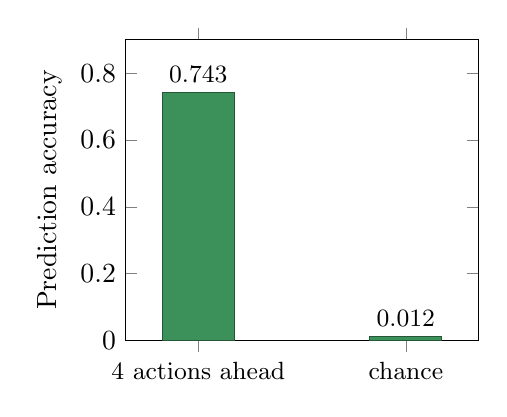
\begin{tikzpicture}
\begin{axis}[
  width=0.5\textwidth, height=5.4cm,
  ybar, bar width=26pt,
  ymin=0, ymax=0.9, enlarge x limits=0.35,
  ylabel={Prediction accuracy},
  symbolic x coords={4 actions ahead, chance},
  xtick=data, x tick label style={font=\small},
  nodes near coords, nodes near coords style={font=\small},
]
\addplot[fill=micagreen, draw=micagreen!60!black] coordinates {
  (4 actions ahead, 0.7433) (chance, 0.0115) };
\end{axis}
\end{tikzpicture}
\caption{\textbf{Not just naming the goal --- predicting the moves.} Every
builder action is written in a fixed vocabulary of 87 possible moves (walk,
turn, place this block, break that one, \ldots). Here the model must predict
the builder's action \emph{four moves into the future}, on sessions kept out
of training. It is right 74\% of the time; blind guessing would be right
1.2\% of the time (the small bar). ``Right'' means the exact move, with a
small tolerance of $\pm2$ blocks on positions. Predicting several moves ahead
is the practical test of understanding: it is what would let a helper prepare
before being asked.
\textit{Source: OBSERVATION --- the predictor is learned entirely from
watching; only the definition of ``right'' is hand-written.}}
\end{figure}

\end{document}
